\subsection{Optimizations for Leiden algorithm}
\label{sec:leiden}

We extend our optimization techniques, originally designed for the Louvain method \cite{sahu2023gvelouvain}, to the Leiden algorithm. Specifically, we implement an \textit{asynchronous} version of the Leiden algorithm, allowing threads to operate independently on distinct sections of the graph. While this approach promotes faster convergence, it also introduces variability into the final result \cite{com-shi21}. To ensure efficient computations, we allocate a dedicated hashtable per thread. These hashtables serve two main purposes: they keep track of the delta-modularity associated with moving to each community connected to a vertex during the local-moving/refinement phases, and they record the total edge weight between super-vertices in the aggregation phase of the algorithm \cite{sahu2023gvelouvain}.

Our optimizations encompass several strategies, including utilizing OpenMP's \textit{dynamic} loop scheduling, capping the number of iterations per pass at $20$, employing a tolerance drop rate of $10$ (threshold scaling), initiating with a tolerance of $0.01$, using an aggregation tolerance of $0.8$ to avoid performing aggregations of minimal utility, implementing flag-based vertex pruning (instead of a queue-based one \cite{nguyenleiden}), utilizing parallel prefix sum, and using preallocated Compressed Sparse Row (CSR) data structures for identifying community vertices and storing the super-vertex graph during aggregation. Additionally, we employ fast collision-free per-thread hashtables, well separated in their memory addresses \cite{sahu2023gvelouvain}.

We attempt two approaches of the Leiden algorithm. One uses a \textit{greedy refinement phase} where vertices greedily optimize for delta-modularity (within their community bounds), while the other uses a \textit{randomized refinement phase} (using fast \textit{xorshift32} random number generators), where the likelihood of selection of a community to move to (by a vertex) is proportional to its delta-modularity, as originally proposed \cite{com-traag19}. Our results, shown in Figures \ref{fig:leidenopt-runtime} and \ref{fig:leidenopt-modularity}, indicate the \textit{greedy approach} performs the best on average, both in terms of runtime and modularity. We also try medium and heavy variants for both approaches, which disables threshold scaling and aggregation tolerance (including threshold scaling) respectively, However, we do not find them to perform well overall.\ignore{On \textit{europe\_osm} graph, our parallel Greedy-Leiden (which we from here on refer to simply as Leiden) runs $3\times$ faster than Nguyen \cite{nguyenleiden}.}

\ignore{We fixed a bug that caused the Leiden algorithm to fail in finding communities on road networks and kmer graphs. The issue was forgetting to reset the affected vertices flags before running the refinement phase.}

\begin{figure}[hbtp]
  \centering
  \subfigure{
    \label{fig:leidenopt-runtime--all}
    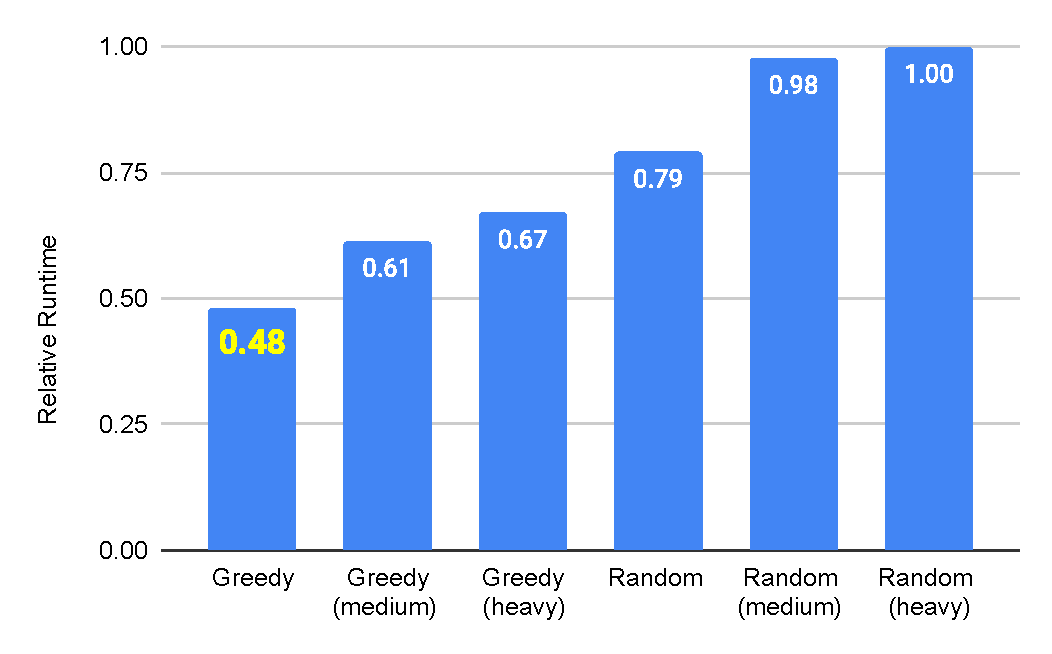
\includegraphics[width=0.98\linewidth]{out/leidenopt-runtime.pdf}
  } \\[-2ex]
  \caption{Average relative runtime for the \textit{greedy} and \textit{random} approaches (including \textit{medium} and \textit{heavy} variants) of parallel Leiden algorithm for all graphs in the dataset.}
  \label{fig:leidenopt-runtime}
\end{figure}

\begin{figure}[hbtp]
  \centering
  \subfigure{
    \label{fig:leidenopt-modularity--all}
    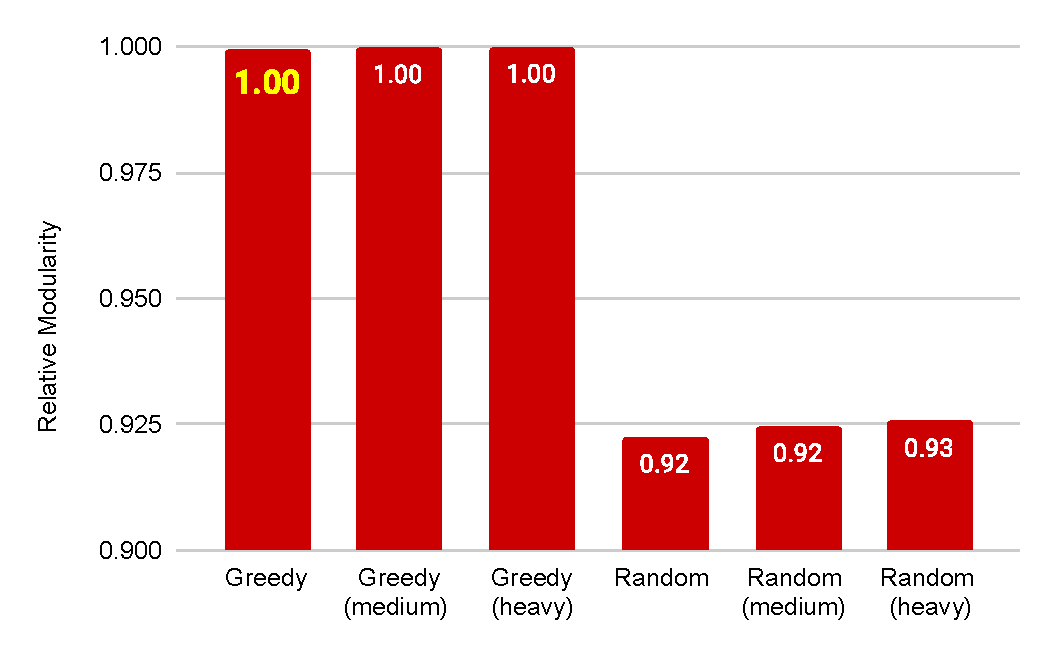
\includegraphics[width=0.98\linewidth]{out/leidenopt-modularity.pdf}
  } \\[-2ex]
  \caption{Average relative modularity for the \textit{greedy} and \textit{random} approaches (including \textit{medium} and \textit{heavy} variants) of parallel Leiden algorithm for all graphs in the dataset.}
  \label{fig:leidenopt-modularity}
\end{figure}

\begin{figure*}[hbtp]
  \centering
  \subfigure{
    \label{fig:leiden-pass--all}
    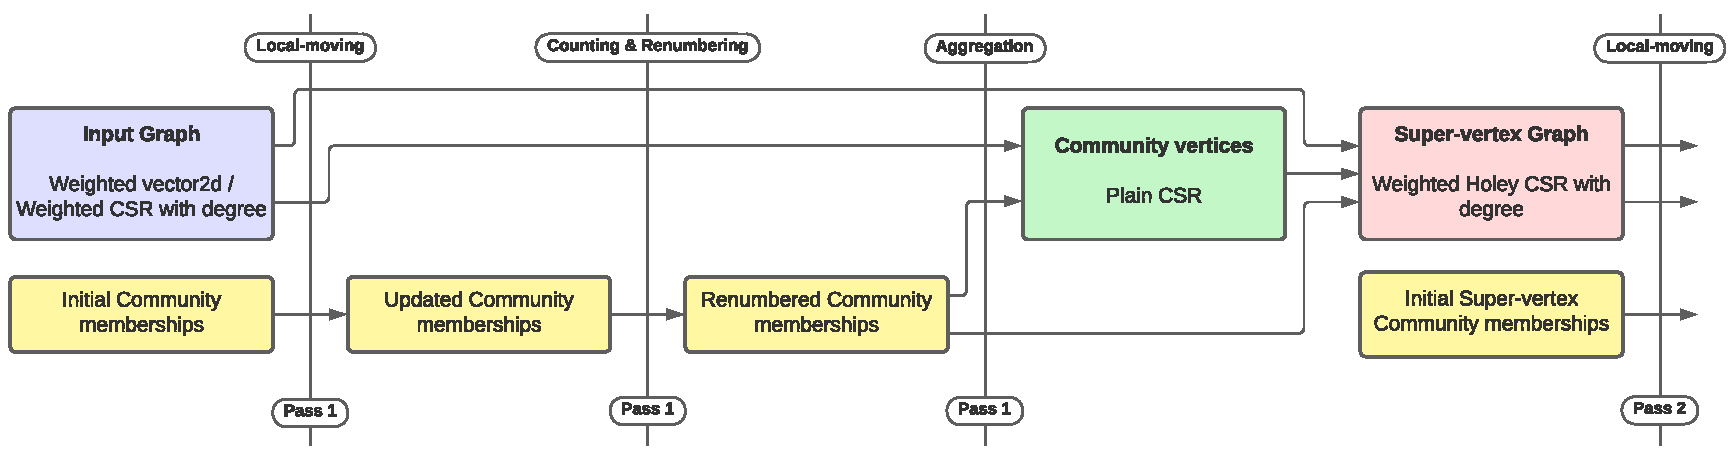
\includegraphics[width=0.98\linewidth]{out/leiden-pass.pdf}
  } \\[-2ex]
  \caption{A flow diagram illustrating the first pass of GVE-Leiden for either a Weighted 2D-vector-based or a Weighted CSR with degree-based input graph. In the local-moving phase, vertex community memberships are updated to obtain community bounds for the refinement phase, until the cumulative delta-modularity change across all vertices reaches a specified threshold. Then, in the refinement phase, the each vertex starts in a singleton community, and community memberships are updated similarly to the local-moving phase, with vertices changing communities within their bounds. These community memberships are then counted and renumbered. In the aggregation phase, community vertices in a CSR are first obtained. This is used to create the super-vertex graph stored in a Weighted Holey CSR with degree. Subsequent passes use a Weighted Holey CSR with degree and initial community memberships for super-vertices from the previous pass as input.}
  \label{fig:leiden-pass}
\end{figure*}





\subsection{Our optimized Leiden implementation}

We now explain the implementation of GVE-Leiden in Algorithms \ref{alg:leiden}, \ref{alg:leidenlm}, \ref{alg:leidenre}, and \ref{alg:leidenag}. A flow diagram illustrating the first pass of GVE-Leiden is shown in Figure \ref{fig:leiden-pass}.


\subsubsection{Main step of GVE-Leiden}

The main step of GVE-Leiden (\texttt{leiden()} function) is outlined in Algorithm \ref{alg:leiden}. It encompasses initialization, the local-moving phase, the refinement phase, and the aggregation phase. Here, the \texttt{leiden()} function accepts the input graph $G$, and returns the community membership $C$ of each vertex. In line \ref{alg:leiden--initialization}, we first initialize the community membership $C$ for each vertex in $G$, and perform passes of the Leiden algorithm, limited to $MAX\_PASSES$ (lines \ref{alg:leiden--passes-begin}-\ref{alg:leiden--passes-end}). During each pass, we initialize the total edge weight of each vertex $K'$, the total edge weight of each community $\Sigma'$, and the community membership $C'$ of each vertex in the current graph $G'$ (line \ref{alg:leiden--reset-weights}).

Subsequently, in line \ref{alg:leiden--local-move}, we perform the local-moving phase by invoking \texttt{leidenMove()} (Algorithm \ref{alg:leidenlm}), which optimizes community assignments. Following this, we set the \textit{community bound} of each vertex (for the refinement phase) as the community membership of each vertex just obtained, and reset the membership of each vertex, and the total weight of each community as singleton vertices in line \ref{alg:leiden--reset-again}. In line \ref{alg:leiden--refine}, the refinement phase is carried out by invoking \texttt{leidenRefine()} (Algorithm \ref{alg:leidenre}), which optimizes the community assignment of each vertex within its community bound. If either the local-moving or the refinement phase converged in a single iteration, global convergence is implied and we terminate the passes (line \ref{alg:leiden--globally-converged}). Further, if the drop in community count $|\Gamma|$ is marginal, we halt at the current pass (line \ref{alg:leiden--aggregation-tolerance}).

If convergence has not been achieved, we proceed to renumber communities (line \ref{alg:leiden--renumber}), update top-level community memberships $C$ with dendrogram lookup (line \ref{alg:leiden--lookup}), perform the aggregation phase by calling \texttt{leidenAggregate()} (Algorithm \ref{alg:leidenag}), and adjust the convergence threshold for subsequent passes, i.e., perform threshold scaling (line \ref{alg:leiden--threshold-scaling}). The next pass commences in line \ref{alg:leiden--passes-begin}. At the end of all passes, we perform a final update of the top-level community memberships $C$ with dendrogram lookup (line \ref{alg:leiden--lookup-last}), and return the top-level community membership $C$ of each vertex in $G$.

\begin{algorithm}[hbtp]
\caption{GVE-Leiden: Our parallel Leiden algorithm.}
\label{alg:leiden}
\begin{algorithmic}[1]
\Require{$G$: Input graph}
\Require{$C$: Community membership of each vertex}
\Require{$G'$: Input/super-vertex graph}
\Require{$C'$: Community membership of each vertex in $G'$}
\Require{$K'$: Total edge weight of each vertex}
\Require{$\Sigma'$: Total edge weight of each community}
\Ensure{$G'_{C'}$: Community vertices (CSR)}
\Ensure{$H_t$: Collision-free per-thread hashtable}
\Ensure{$l_i$, $l_j$: Number of iterations performed (per pass)}
\Ensure{$l_p$: Number of passes performed}
\Ensure{$\tau$: Per iteration tolerance}
\Ensure{$\tau_{agg}$: Aggregation tolerance}

\Statex

\Function{leiden}{$G$} \label{alg:leiden--begin}
  \State Vertex membership: $C \gets [0 .. |V|)$ \textbf{;} $G' \gets G$ \label{alg:leiden--initialization}
  \ForAll{$l_p \in [0 .. \text{\small{MAX\_PASSES}})$} \label{alg:leiden--passes-begin}
    \State $\Sigma' \gets K' \gets vertexWeights(G')$ \textbf{;} $C' \gets [0 .. |V'|)$ \label{alg:leiden--reset-weights}
    \State $l_i \gets leidenMove(G', C', K', \Sigma', \tau)$ \Comment{Alg. \ref{alg:leidenlm}} \label{alg:leiden--local-move}
    \State $C'_B \gets C'$ \textbf{;} $C' \gets [0 .. |V'|)$ \textbf{;} $\Sigma' \gets K'$ \label{alg:leiden--reset-again}
    \State $l_j \gets leidenRefine(G', C'_B, C', K', \Sigma', \tau)$ \Comment{Alg. \ref{alg:leidenre}} \label{alg:leiden--refine}
    \If{$l_i + l_j \le 1$} \textbf{break} \Comment{Globally converged?} \label{alg:leiden--globally-converged}
    \EndIf
    \State $|\Gamma|, |\Gamma_{old}| \gets$ Number of communities in $C$, $C'$
    \If{$|\Gamma|/|\Gamma_{old}| > \tau_{agg}$} \textbf{break} \Comment{Low shrink?} \label{alg:leiden--aggregation-tolerance}
    \EndIf
    \State $C' \gets$ Renumber communities in $C'$ \label{alg:leiden--renumber}
    \State $C \gets$ Lookup dendrogram using $C$ to $C'$ \label{alg:leiden--lookup}
    \State $G' \gets leidenAggregate(G', C')$ \Comment{Alg. \ref{alg:leidenag}} \label{alg:leiden--aggregate}
    \State $C' \gets$ Map $C'$ to $C'_B$ \Comment{Use move-based membership} \label{alg:leiden--useparent}
    \State $\tau \gets \tau / \text{\small{TOLERANCE\_DROP}}$ \Comment{Threshold scaling} \label{alg:leiden--threshold-scaling}
  \EndFor \label{alg:leiden--passes-end}
  \State $C \gets$ Lookup dendrogram using $C$ to $C'$ \label{alg:leiden--lookup-last}
  \Return{$C$} \label{alg:leiden--return}
\EndFunction \label{alg:leiden--end}
\end{algorithmic}
\end{algorithm}

\begin{algorithm}[hbtp]
\caption{Local-moving phase of GVE-Leiden.}
\label{alg:leidenlm}
\begin{algorithmic}[1]
\Require{$G'$: Input/super-vertex graph}
\Require{$C'$: Community membership of each vertex}
\Require{$K'$: Total edge weight of each vertex}
\Require{$\Sigma'$: Total edge weight of each community}
\Ensure{$G'_{C'}$: Community vertices (CSR)}
\Ensure{$H_t$: Collision-free per-thread hashtable}
\Ensure{$l_i$: Number of iterations performed}
\Ensure{$\tau$: Per iteration tolerance}

\Statex

\Function{leidenMove}{$G', C', K', \Sigma', \tau$} \label{alg:leidenlm--move-begin}
  \State Mark all vertices in $G'$ as unprocessed \label{alg:leidenlm--reset-affected}
  \ForAll{$l_i \in [0 .. \text{\small{MAX\_ITERATIONS}})$} \label{alg:leidenlm--iterations-begin}
    \State Total delta-modularity per iteration: $\Delta Q \gets 0$ \label{alg:leidenlm--init-deltaq}
    \ForAll{unprocessed $i \in V'$ \textbf{in parallel}} \label{alg:leidenlm--loop-vertices-begin}
      \State Mark $i$ as processed (prune) \label{alg:leidenlm--prune}
      \State $H_t \gets scanCommunities(\{\}, G', C', i, false)$ \label{alg:leidenlm--scan}
      \State $\rhd$ Use $H_t, K', \Sigma'$ to choose best community
      \State $c^* \gets$ Best community linked to $i$ in $G'$ \label{alg:leidenlm--best-community-begin}
      \State $\delta Q^* \gets$ Delta-modularity of moving $i$ to $c^*$ \label{alg:leidenlm--best-community-end}
      \If{$c^* = C'[i]$} \textbf{continue} \label{alg:leidenlm--best-community-same}
      \EndIf
      \State $\Sigma'[C'[i]] -= K'[i]$ \textbf{;} $\Sigma'[c^*] += K'[i]$ \textbf{atomic} \label{alg:leidenlm--perform-move-begin}
      \State $C'[i] \gets c^*$ \textbf{;} $\Delta Q \gets \Delta Q + \delta Q^*$ \label{alg:leidenlm--perform-move-end}
      \State Mark neighbors of $i$ as unprocessed \label{alg:leidenlm--remark}
    \EndFor \label{alg:leidenlm--loop-vertices-end}
    \If{$\Delta Q \le \tau$} \textbf{break} \Comment{Locally converged?} \label{alg:leidenlm--locally-converged}
    \EndIf
  \EndFor \label{alg:leidenlm--iterations-end}
  \Return{$l_i$} \label{alg:leidenlm--return}
\EndFunction \label{alg:leidenlm--move-end}

\Statex

\Function{scanCommunities}{$H_t, G', C', i, self$}
  \ForAll{$(j, w) \in G'.edges(i)$}
    \If{\textbf{not} $self$ \textbf{and} $i = j$} \textbf{continue}
    \EndIf
    \State $H_t[C'[j]] \gets H_t[C'[j]] + w$
  \EndFor
  \Return{$H_t$}
\EndFunction
\end{algorithmic}
\end{algorithm}

\begin{algorithm}[hbtp]
\caption{Refinement phase of GVE-Leiden.}
\label{alg:leidenre}
\begin{algorithmic}[1]
\Require{$G'$: Input/super-vertex graph}
\Require{$C'$: Community membership of each vertex}
\Require{$K'$: Total edge weight of each vertex}
\Require{$\Sigma'$: Total edge weight of each community}
\Ensure{$G'_{C'}$: Community vertices (CSR)}
\Ensure{$H_t$: Collision-free per-thread hashtable}
\Ensure{$\tau$: Per iteration tolerance}

\Statex

\Function{leidenRefine}{$G', C'_B, C', K', \Sigma', \tau$} \label{alg:leidenre--move-begin}
  \ForAll{$i \in V'$ \textbf{in parallel}} \label{alg:leidenre--loop-vertices-begin}
    \If{$\Sigma'[C'[i]] \neq K'[i]$} \textbf{continue} \label{alg:leidenre--check-isolated}
    \EndIf
    \State $H_t \gets scanBounded(\{\}, G', C'_B, C', i, false)$ \label{alg:leidenre--scan}
    \State $\rhd$ Use $H_t, K', \Sigma'$ to choose best community
    \State $c^* \gets$ Best community linked to $i$ in $G'$ within $C'_B$ \label{alg:leidenre--best-community-begin}
    \State $\delta Q^* \gets$ Delta-modularity of moving $i$ to $c^*$ \label{alg:leidenre--best-community-end}
    \If{$c^* = C'[i]$} \textbf{continue} \label{alg:leidenre--best-community-same}
    \EndIf
    \If{$atomicCAS(\Sigma'[C'[i]], 0) = K'[C'[i]]$} \label{alg:leidenre--perform-move-begin}
      \State $\Sigma'[c^*] += K'[i]$ \textbf{atomically}
      \State $C'[i] \gets c^*$ \label{alg:leidenre--perform-move-end}
    \EndIf
  \EndFor \label{alg:leidenre--loop-vertices-end}
\EndFunction \label{alg:leidenre--move-end}

\Statex

\Function{scanBounded}{$H_t, G', C'_B, C', i, self$}
  \ForAll{$(j, w) \in G'.edges(i)$}
    \If{\textbf{not} $self$ \textbf{and} $i = j$} \textbf{continue}
    \EndIf
    \If{$C'_B[i] \neq C'_B[j]$} \textbf{continue}
    \EndIf
    \State $H_t[C'[j]] \gets H_t[C'[j]] + w$
  \EndFor
  \Return{$H_t$}
\EndFunction

\Statex

\Function{atomicCAS}{$pointer, old, new$}
  \State $\rhd$ Perform the following atomically
  \If{$pointer = old$} $pointer \gets new$ \textbf{;} \ReturnInline{$old$}
  \Else\ \ReturnInline{$pointer$}
  \EndIf
\EndFunction
\end{algorithmic}
\end{algorithm}

\begin{algorithm}[hbtp]
\caption{Aggregation phase of GVE-Leiden.}
\label{alg:leidenag}
\begin{algorithmic}[1]
\Require{$G'$: Input/super-vertex graph}
\Require{$C'$: Community membership of each vertex}
\Ensure{$G'_{C'}$: Community vertices (CSR)}
\Ensure{$G''$: Super-vertex graph (weighted CSR)}
\Ensure{$*.offsets$: Offsets array of a CSR graph}
\Ensure{$H_t$: Collision-free per-thread hashtable}

\Statex

\Function{leidenAggregate}{$G', C'$}
  \State $\rhd$ Obtain vertices belonging to each community
  \State $G'_{C'}.offsets \gets countCommunityVertices(G', C')$ \label{alg:leidenag--coff-begin}
  \State $G'_{C'}.offsets \gets exclusiveScan(G'_{C'}.offsets)$ \label{alg:leidenag--coff-end}
  \ForAll{$i \in V'$ \textbf{in parallel}} \label{alg:leidenag--comv-begin}
    \State Add edge $(C'[i], i)$ to CSR $G'_{C'}$ \textbf{atomically}
  \EndFor \label{alg:leidenag--comv-end}
  \State $\rhd$ Obtain super-vertex graph
  \State $G''.offsets \gets communityTotalDegree(G', C')$ \label{alg:leidenag--yoff-begin}
  \State $G''.offsets \gets exclusiveScan(G''.offsets)$ \label{alg:leidenag--yoff-end}
  \State $|\Gamma| \gets$ Number of communities in $C'$
  \ForAll{$c \in [0, |\Gamma|)$ \textbf{in parallel}} \label{alg:leidenag--y-begin}
    % \If{degree of $c$ in $G'_{C'} = 0$} \textbf{continue}
    % \EndIf
    \State $H_t \gets \{\}$
    \ForAll{$i \in G'_{C'}.edges(c)$}
      \State $H_t \gets scanCommunities(H_t, G', C', i, true)$
    \EndFor
    \ForAll{$(d, w) \in H_t$}
      \State Add edge $(c, d, w)$ to CSR $G''$ \textbf{atomically}
    \EndFor
  \EndFor \label{alg:leidenag--y-end}
  \Return $G''$ \label{alg:leidenag--return}
\EndFunction
\end{algorithmic}
\end{algorithm}



\subsubsection{Local-moving phase of GVE-Leiden}

The pseuodocode for the local-moving phase of GVE-Leiden is shown in Algorithm \ref{alg:leidenlm}, which iteratively moves vertices between communities to maximize modularity. Here, the \texttt{leidenMove()} function takes the current graph $G'$, community membership $C'$, total edge weight of each vertex $K'$ and each community $\Sigma'$, the iteration tolerance $\tau$ as input, and returns the number of iterations performed $l_i$.

Lines \ref{alg:leidenlm--iterations-begin}-\ref{alg:leidenlm--iterations-end} represent the main loop of the local-moving phase. In line \ref{alg:leidenlm--reset-affected}, we first mark all vertices as unprocessed. Then, in line \ref{alg:leidenlm--init-deltaq}, we initialize the total delta-modularity per iteration $\Delta Q$. Next, in lines \ref{alg:leidenlm--loop-vertices-begin}-\ref{alg:leidenlm--loop-vertices-end}, we iterate over unprocessed vertices in parallel. For each unprocessed vertex $i$, we mark $i$ as processed - vertex pruning (line \ref{alg:leidenlm--prune}), scan communities connected to $i$ - excluding self (line \ref{alg:leidenlm--scan}), determine the best community $c*$ to move $i$ to (line \ref{alg:leidenlm--best-community-begin}), and calculate the delta-modularity of moving $i$ to $c*$ (line \ref{alg:leidenlm--best-community-end}). We then update the community membership of $i$ (lines \ref{alg:leidenlm--perform-move-begin}-\ref{alg:leidenlm--perform-move-end}) and mark its neighbors as unprocessed (line \ref{alg:leidenlm--remark}) if a better community was found. In line \ref{alg:leidenlm--locally-converged}, we check if the local-moving phase has converged. If so, we break out of the loop (or if $MAX\_ITERATIONS$ is reached). At the end, in line \ref{alg:leidenlm--return}, we return the number of iterations performed $l_i$.


\subsubsection{Refinement phase of GVE-Leiden}

The pseuodocode for the refinement phase of GVE-Leiden is presented in Algorithm \ref{alg:leidenlm}. This is similar to the local-moving phase, but utilizes the obtained community membership of each vertex as a \textit{community bound}, where each vertex must choose to join the community of another vertex within its community bound.\ignore{Similar to the local-moving phase however, vertices iteratively move between communities to maximize modularity.} At the start of the refinement phase, the community membership of each vertex is reset, such that each vertex belongs to its own community. Here, the \texttt{leidenRefine()} function takes the current graph $G'$, the community bound of each vertex $C'_B$, the initial community membership $C'$ of each vertex, the total edge weight of each vertex $K'$, the initial total edge weight of each community $\Sigma'$, and the current per iteration tolerance $\tau$ as input, and returns the number of iterations performed $l_j$.

Lines \ref{alg:leidenre--iterations-begin}-\ref{alg:leidenre--iterations-end} represent the core of the refinement phase. First, we initialize all vertices as unprocessed (line \ref{alg:leidenre--reset-affected}). Subsequently, we initialize the per-iteration delta-modularity $\Delta Q$ (line \ref{alg:leidenre--init-deltaq}), and iterate over unprocessed vertices in parallel (lines \ref{alg:leidenre--loop-vertices-begin}-\ref{alg:leidenre--loop-vertices-end}). For each unprocessed vertex $i$, we prune $i$ (line \ref{alg:leidenre--prune}), scan communities connected to $i$ within the \textit{same community bound} - excluding self (line \ref{alg:leidenre--scan}), evaluate the best community $c*$ to move $i$ to (line \ref{alg:leidenre--best-community-begin}), and compute the delta-modularity of moving $i$ to $c*$ (line \ref{alg:leidenre--best-community-end}). If a better community was found, we update the community membership (lines \ref{alg:leidenre--perform-move-begin}-\ref{alg:leidenre--perform-move-end}) of $i$, and mark its neighbors as unprocessed (line \ref{alg:leidenre--remark}). In line \ref{alg:leidenre--locally-converged}, we check if the refinement phase has converged. If so, we stop iterating (or if $MAX\_ITERATIONS$ is reached). Finally, we return the number of iterations performed $l_j$ (line \ref{alg:leidenre--return}).

\begin{algorithm}[hbtp]
\caption{Finding disconnected communities in parallel.}
\label{alg:disconnected}
\begin{algorithmic}[1]
\Require{$G$: Input graph}
\Require{$C$: Community membership of each vertex}
\Ensure{$D$: Disconnected flag for each community}
\Ensure{$S$: Size of each community}
\Ensure{$f_{if}$: Perform BFS to vertex $j$ if condition satisfied}
\Ensure{$f_{do}$: Perform operation after each vertex is visited}
\Ensure{$reached$: Number of vertices reachable from $i$ to $i$'s community}
\Ensure{$work_t$: Work-list of current thread}

\Statex

\Function{disconnectedCommunities}{$G, C$} \label{alg:disconnected--begin}
  \State $D \gets \{\}$ \textbf{;} $vis \gets \{\}$ \label{alg:disconnected--init}
  \State $S \gets communitySizes(G, C)$ \label{alg:disconnected--sizes}
  \ForAll{\textbf{threads in parallel}} \label{alg:disconnected--threads-begin}
    \ForAll{$i \in V$} \label{alg:disconnected--loop-begin}
      \State $c \gets C[i]$ \textbf{;} $reached \gets 0$ \label{alg:disconnected--unreached}
      \State $\rhd$ Skip if community $c$ is empty, or
      \State $\rhd$ does not belong to work-list of current thread.
      \If{$S[c] = 0$ \textbf{or} $c \notin work_t$} \textbf{continue} \label{alg:disconnected--work}
      \EndIf
      \State $f_{if} \gets (j) \implies C[j] = c$
      \State $f_{do} \gets (j) \implies reached \gets reached + 1$
      \State $bfsVisitForEach(vis, G, i, f_{if}, f_{do})$ \label{alg:disconnected--bfs}
      \If{$reached < S[c]$} $D[c] \gets 1$ \label{alg:disconnected--mark}
      \EndIf
      \State $S[c] \gets 0$ \label{alg:disconnected--processed}
    \EndFor \label{alg:disconnected--loop-end}
  \EndFor \label{alg:disconnected--threads-end}
  \Return{$D$}
\EndFunction \label{alg:disconnected--end}
\end{algorithmic}
\end{algorithm}



\subsubsection{Aggregation phase of GVE-Leiden}

Finally, we show the psuedocode for the aggregation phase in Algorithm \ref{alg:leidenag}, where communities are aggregated into super-vertices in preparation for the next pass of the Leiden algorithm (which operates on the super-vertex graph). Here, the \texttt{leidenAggregate()} function takes the current graph $G'$ and the community membership $C'$ as input, and returns the super-vertex graph $G''$.

In lines \ref{alg:leidenag--coff-begin}-\ref{alg:leidenag--coff-end}, the offsets array for the community vertices CSR $G'_{C'}.offsets$ is obtained. This is achieved by initially counting the number of vertices in each community using \texttt{countCommunityVert} \texttt{ices()} and subsequently performing an exclusive scan on the array. In lines \ref{alg:leidenag--comv-begin}-\ref{alg:leidenag--comv-end},  a parallel iteration over all vertices is performed to atomically populate vertices belonging to each community into the community graph CSR $G'_{C'}$. Following this, the offsets array for the super-vertex graph CSR is obtained by overestimating the degree of each super-vertex. This involves calculating the total degree of each community with \texttt{communityTotalDegree()} and performing an exclusive scan on the array (lines \ref{alg:leidenag--yoff-begin}-\ref{alg:leidenag--yoff-end}). As a result, the super-vertex graph CSR becomes holey, featuring gaps between the edges and weights arrays of each super-vertex in the CSR.

Then, in lines \ref{alg:leidenag--y-begin}-\ref{alg:leidenag--y-end}, a parallel iteration over all communities $c \in [0, |\Gamma|)$ is performed. For each vertex $i$ belonging to community $c$, all communities $d$ (with associated edge weight $w$), linked to $i$ as defined by \texttt{scanCommunities()} in Algorithm \ref{alg:leidenlm}, are added to the per-thread hashtable $H_t$. Once $H_t$ is populated with all communities (and associated weights) linked to community $c$, these are atomically added as edges to super-vertex $c$ in the super-vertex graph $G''$. Finally, in line \ref{alg:leidenag--return}, we return the super-vertex graph $G''$.




\subsection{Finding disconnected communities}

We now outline our parallel algorithm for identifying disconnected communities, given the original graph and the community membership of each vertex. The core concept involves determining the size of each community, selecting a vertex from each community, traversing within the community from that vertex (avoiding adjacent communities), and marking a community as disconnected if all its vertices cannot be reached. We explore four distinct approaches, differing in the use of parallel Depth-First Search (DFS) or Breadth-First Search (BFS) and whether per-thread or shared \textit{visited} flags are employed. If shared visited flags are used, each thread scans all vertices but processes only its assigned community based on the community ID. Our findings suggest that utilizing parallel BFS traversal with a shared flag vector yields the fastest results. As this is not a heuristic algorithm, all approaches produce identical outcomes. Algorithm \ref{alg:disconnected} illustrates the pseudocode for this approach. Here, the \texttt{disconnectedCommunities()} function takes the input graph $G$ and the community membership $C$ as input, and it returns the disconnected flag $D$ for each community.

We now explain Algorithm \ref{alg:disconnected} in detail. First, in line \ref{alg:disconnected--init}, the disconnected community flag $D$, and the visited vertices flags $vis$ are initialized. In line \ref{alg:disconnected--sizes}, the size of each community $S$ is obtained in parallel using the \texttt{communitySizes()} function. Subsequently, each thread processes each vertex $i$ in the graph $G$ in parallel (lines \ref{alg:disconnected--loop-begin}-\ref{alg:disconnected--loop-end}). In line \ref{alg:disconnected--unreached}, the community membership of $i$ ($c$) is determined, and the count of vertices reached from $i$ is initialized to $0$. If community $c$ is empty or not in the work-list of the current thread $work_t$, the thread proceeds to the next iteration (line \ref{alg:disconnected--work}). If however the community $c$ is non-empty and in the work-list of the current thread $work_t$, BFS is performed from vertex $i$ to explore vertices in the same community, using lambda functions $f_{if}$ to conditionally perform BFS to vertex $j$ if it belongs to the same community, and $f_{do}$ to update the count of $reached$ vertices after each vertex is visited during BFS (line \ref{alg:disconnected--bfs}). If the number of vertices $reached$ during BFS is less than the community size $S[c]$, the community $c$ is marked as disconnected (line \ref{alg:disconnected--mark}). Finally, the size of the community $S[c]$ is updated to $0$, indicating that the community has been processed (line \ref{alg:disconnected--processed}). Note that the work-list $work_t$ for each thread with ID $t$, is defined as a set containing communities $[t\chi,\ t(\chi+1))\ \cup\ [T\chi + t\chi,\ T\chi + t(\chi+1))\ \cup\ \ldots$, where $\chi$ is the chunk size, and $T$ is the number of threads. We use a chunk size of $\chi = 1024$.
